\centerline{\LARGE{\textbf{Assignment 3: Intrusion Analysis}}}
\setcounter{section}{0}
\section{Introduction}
On April 28, 2023, the IT department at DSV received a concerning notification from the national computer emergency response team (CERT-SE) regarding potential unauthorized activity within the network infrastructure. The alert indicated unusual activity targeting one or more computers, with specific reference to the development test server of the Haisy student management and grade database system. 

\noindent\rule{\textwidth}{1pt}
\vspace{-0.8cm}
\begin{verbatim}
Date: Tues, 28 Apr 2023 11:29:03 +0100
From: CERT-SE <alert@cert.se>
To: CS2Lab <cs2lab@dsv.su.se>
Subject: Important Information from CERT-SE: Indications of Intrusion Attempt

CERT-SE has noticed unusual activity against one or more computers
in your network. See details below.

IP: 193.10.9.5
Computer name: haisy.cs2lab.dsv.su.se
Attack type: Possible intrusion attempt
Time, from circa: 2023-04-27 23:50:25 CET

Sincerely
CERT-SE	
\end{verbatim}
\vspace{-0.5cm}
\noindent\rule{\textwidth}{1pt}
\vspace{0cm}

\noindent As part of the responsibility to maintain the security and integrity of the systems, an investigation to ascertain the nature and extent of the incident was initiated. The Haisy development test server, hosted at haisy.cs2lab.dsv.su.se, is a critical component of the infrastructure, supporting the ongoing development and testing of the Haisy system, which manages student data and academic records. Any compromise to this system could have significant ramifications for the confidentiality, integrity, and availability of sensitive information.
\newline

\noindent This report documents our investigation into the potential network intrusion, with the objective of understanding the events leading up to the alert from CERT-SE, identifying any unauthorized access or malicious activity, and assessing the impact on our systems and data. By conducting a thorough analysis of the available evidence and applying appropriate forensic techniques, we aim to provide actionable insights to mitigate risks, enhance security measures, and prevent future incidents of this nature.
\newpage
\section{Methods}
Our investigation into the possible network intrusion targeting the Haisy development test server began with a thorough confirmation of the integrity of the provided evidence files: \texttt{haisy\_4000.pcap} and \texttt{haisy.raw}. We utilized their respective SHA1 and MD5 hash values to ensure that the files had not been altered or corrupted since their acquisition.

\paragraph{Method and Tools for Analysing the Network Traffic}\mbox{}\\
\noindent\rule{\textwidth}{1pt}
\vspace{-0.8cm}
\begin{table}[h]
\begin{tabular}{ll}
Kali Linux (VM) & \texttt{2024.1}                                 \\
Wireshark      & \texttt{wireshark:amd64/kali-rolling 4.2.2-1} \\
Geo Data Tool   & \texttt{https://www.geodatatool.com/en/}  (last accessed on April 28, 2024)
\end{tabular}
\end{table}

\vspace{-0.8cm}
\noindent\rule{\textwidth}{1pt}
\vspace{-0.3cm}

\noindent We proceeded to analyze the \texttt{haisy\_4000.pcap} file using a Kali 2024.1 virtual machine (VM) equipped with Wireshark 4.2.2. Our primary goal was to gain insight into the network traffic associated with the suspected intrusion. We began our analysis by identifying the number of IP addresses involved in the traffic and examining the source and destination IP addresses. We also attempted to determine which ports were experiencing the highest volume of traffic, which would provide insight into the nature of the communication. We also used the geolocation tool \texttt{https://www.geodatatool.com/en/} to determine the geographic location of the identified IP addresses. This contextual information helped us understand the potential origin or source of the suspicious network activity. Throughout our analysis, we meticulously examined DNS and HTTP packets, as well as TCP streams, looking for any indicators of compromise or anomalous behavior that might indicate an attempted network intrusion.

\paragraph{Method and Tools for Analysing the Linux Server Image}\mbox{}\\
\noindent\rule{\textwidth}{1pt}
\vspace{-0.8cm}
\begin{table}[h]
\begin{tabular}{ll}
Windows 10 (VM) & \texttt{10.0.19045 (Build 19045)}                                 \\
Autopsy      & \texttt{4.21.0}
\end{tabular}
\end{table}

\vspace{-0.8cm}
\noindent\rule{\textwidth}{1pt}
\vspace{-0.3cm}

\noindent We then turned our attention to examining the \texttt{haisy.raw} file in a Windows 10 environment running Autopsy 4.21.0. The goal of this phase of the investigation was to delve deeper into the system-level activity during the incident. Our analysis covered several key areas, including user account management, command execution, and software usage. We began by identifying existing users on the system and examining their account activity for signs of unauthorized access or suspicious behavior. At the same time, we analyzed the commands executed during the relevant time period to identify any anomalies or indicators of malicious activity. In addition, we evaluated the services running on the system at the time of the incident to assess their relevance to the investigation and potential impact on system security. To supplement our analysis, we examined specific log files associated with the running services, focusing on events and activities that could provide evidence of a potential attack or compromise. By meticulously reviewing the system logs, we aimed to uncover any traces of unauthorized access, privilege escalation, or suspicious activity indicative of a network intrusion. Finally, we synthesized the results to construct a comprehensive timeline of events related to the suspected intrusion. This timeline provided a chronological sequence of activities leading up to and during the incident, allowing us to gain a clear understanding of the nature and scope of the attempted intrusion.
\section{Results}
\subsection{Investigating the Network Traffic}
\begin{verbatim}
$ sha1sum haisy_4000.pcap             
5d50246cd8ed94b9d39d60b4008a2ead1e3cba50  haisy_4000.pcap

$ md5sum haisy_4000.pcap 
8f7f17adf4de26e88dd2841dca174b02  haisy_4000.pcap

$ ls -l haisy_4000.pcap 
-rw-r--r-- 1 kali kali 35116793 Apr 23 08:20 haisy_4000.pcap
\end{verbatim}
The verification of the SHA1 and MD5 hash values of the evidence file \texttt{haisy\_4000.pcap} has shown that the file had not been altered or corrupted since its acquisition because the hash values match the values specified in the instructions. The file has a size of 35.1168MB.

\begin{figure}[h]
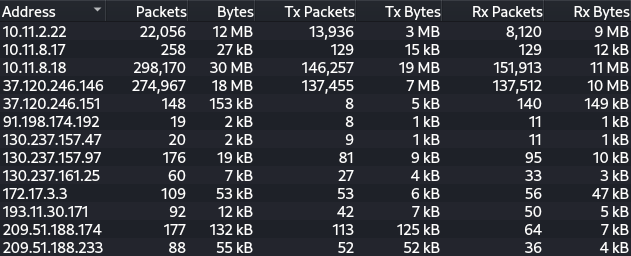
\includegraphics[width=\textwidth]{ip_addresses.png}
\centering
\caption{Statistics $>$ Endpoints $>$ IPv4}
\label{screen:ip_addresses}
\end{figure}

\noindent The file \texttt{haisy\_4000.pcap} contains 300338 captured network packets in total and 13 unique IP addresses occur. Of these IP addresses, 10.11.8.18 (146k transmitted packets, 151k received packets), 37.120.246.146 (137k transmitted packets, 137k received packets), 10.11.2.22 (14k transmitted packets, 8k received packets), 10.11.8.17 (129 transmitted packets, 129 received packets), 209.51.188.174 (113 transmitted packets, 64 received packets) and 130.237.157.97 (8 transmitted packets, 140 received packets) generated the most traffic. The two internal IP addresses that occur most frequently (10.11.8.18 and 10.11.2.22) are the Linux server hosting \url{haisy.cs2lab.dsv.su.se} and the reverse proxy. The top five ports for Linux server (10.11.8.18) are 80, 59808, 42250, 44779, 44216 and for the reverse proxy (10.11.2.22) are 33688, 42598, 49402, 39140, 48330. The only port used for 37.120.246.146 is 60836. 
\newline

\noindent The three most common external IPs can be traced back geographically to Romania, Bucharest (37.120.246.146), United States, Boston (209.51.188.174) and Sweden, Stockholm (130.237.157.97).
\newline

\noindent When looking at the DNS related packets, it is noticeable that attempts were made to call domains that do not exist. For example, attempts were made to call up www.daisy.dsv.su.se or www.daisy.dsv.su.se.cs2lab.dsv.su.se. Domains such as fr.wikipedia.org or fsf.org, which have nothing directly to do with the daisy service, were called. In addition, there are DNS queries resolving to CNAME records such as mimas.dsv.su.se. CNAME records are used to alias one name to another. The presence of CNAME records isn't unusual, but it's important to verify that these canonical names are legitimate and expected within the network environment.

\begin{figure}[h]
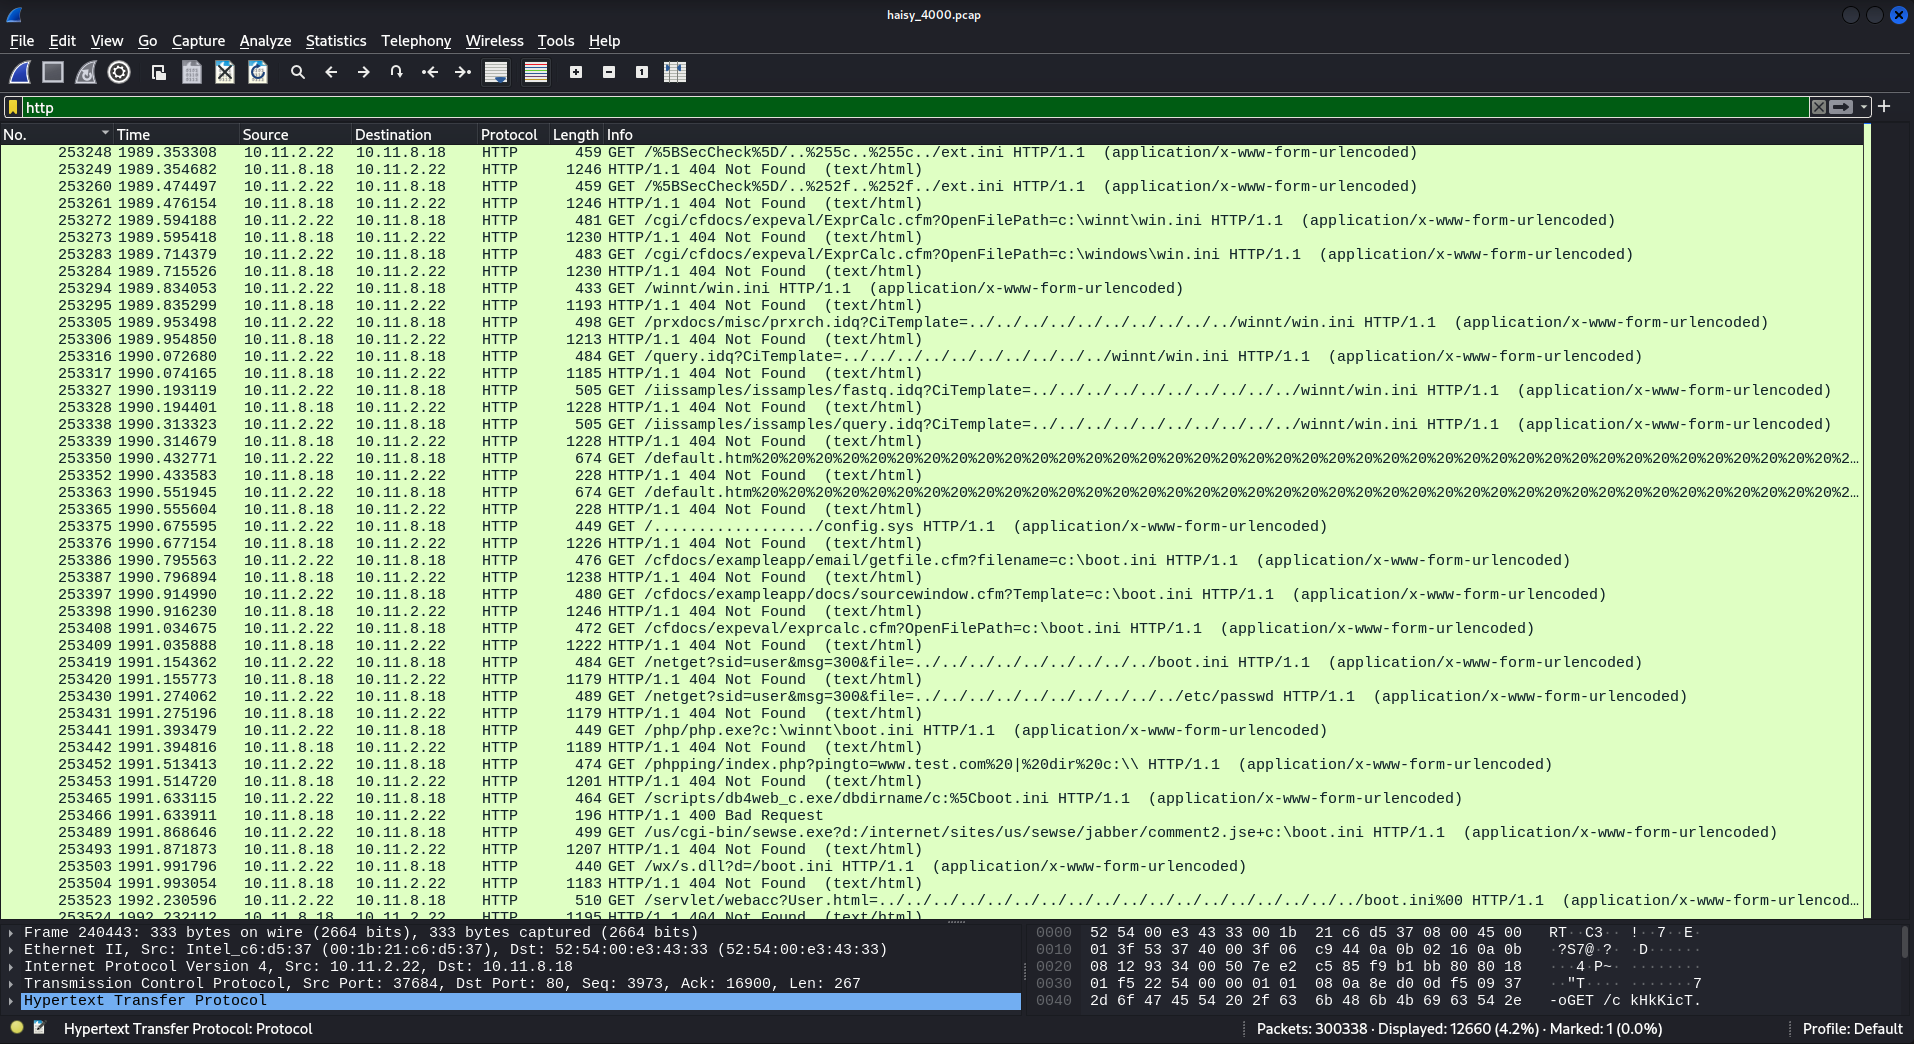
\includegraphics[width=\textwidth]{http_traffic.png}
\centering
\caption{Filter "http"}
\label{screen:http_traffic}
\end{figure}

\noindent When looking at the HTTP traffic, it is noticeable that many GET requests were made to url paths that do not exist. For example, attempts were made to call \url{/iissamples/issamples/fastq.idq?CiTemplate=../../../../../../../../../../../../winnt/win.ini}, \url{/readme.html} or \url{/admin.html} on the Linux server (10.11.8.18). This could be a sign that an attacker tried a directory/path traversal attack.

\subsection{Investigating the Linux Server Image}
\begin{verbatim}
$ sha1sum haisy.raw      
6d08e3ec0c3caac2979070913010c1753c48f66f  haisy.raw

$ md5sum haisy.raw      
89fd1b9b40f2b7793440a4a13d045837  haisy.raw

$ ls -l haisy.raw     
-rw-r--r-- 1 kali kali 16106127360 Apr 23 09:21 haisy.raw
\end{verbatim}
The verification of the SHA1 and MD5 hash values of \texttt{haisy.raw} has shown that the file had not been altered or corrupted since its acquisition because the hash values match the values specified in the instructions. The file has a size of 16.1061GB. The image contains 5 partitions and the operating system according to the lsb-release file is Ubuntu 13.10 codename saucy.
\begin{verbatim}
​​root:x:0:0:root:/root:/bin/bash
daemon:x:1:1:daemon:/usr/sbin:/bin/sh
bin:x:2:2:bin:/bin:/bin/sh
sys:x:3:3:sys:/dev:/bin/sh
sync:x:4:65534:sync:/bin:/bin/sync
games:x:5:60:games:/usr/games:/bin/sh
(...)
postgres:x:107:114:PostgreSQL administrator,,,:/var/lib/postgresql:/bin/bash
whoopsie:x:108:115::/nonexistent:/bin/false
tomcat7:x:109:117::/usr/share/tomcat7:/bin/false
erika:x:1000:1000:Erika Thuning,,,:/home/erika:/bin/bash
\end{verbatim}
\noindent The file \texttt{etc/passwd} contains entries for 29 user accounts whereby a home directory exists only for the user erika. The \texttt{.bash\_history} of the user erika reveals several activities that could be considered suspicious:
\begin{itemize}
	\item Repeated SSH Service Commands (\texttt{sudo /etc/init.d/ssh status, sudo status  /etc/i\\nit.d/ssh, sudo start  /etc/init.d/ssh, sudo  /etc/init.d/ssh}): The frequent stopping, starting, and status checking of the SSH service could indicate trouble with the SSH service, or it might suggest that someone was trying to gain persistent access.
	\item Network Interface Cycling (\texttt{sudo ifconfig eth0 down, sudo ifconfig eth0 up, ...}): Regularly bringing the network interface eth0 down and back up is unusual and could be an attempt to evade network monitoring or reset network connections after unauthorized activities.
	\item Bypassing SSL Certificate Verification (\texttt{wget --no-check-certificate http://daisy.dsv.\\su.se, wget --no-check-certificate dsv.su.se, ...}): The use of --no-check-certificate with wget could suggest And HTTP (no encryption) is used.
	\item Editing Apache Configuration Files (\texttt{nano /etc/apache2/apache2.conf, cd /etc/apache2/, nano apache2.conf, ...}): Changes to the Apache configuration could be legitimate, but they can also indicate an attempt to alter the web server's behavior for malicious purposes, such as setting up a reverse proxy for traffic redirection.
	\item Direct Interaction with MySQL Database (\texttt{mysql -u erika -p < haisy\_students\_2023.sql, mysql -u root -p haisy < haisy\_students\_2023.sql, ...}): Importing/exporting data using the MySQL command line with root access can be a standard administrative task, but it can also be a way to inject malicious data or exfiltrate information.
\end{itemize}
Examination of \texttt{/var/log/syslog} shows that routine tasks such as DHCP renewals and periodic cron jobs were executed. Nevertheless, several segfaults occurred at different times. Segfaults indicate that a program has attempted to access memory for which it did not have permission, or that it has attempted to execute a process that was not allowed. The affected processes include QIRCKvwYm, oymZYryK, wbMEAsyiwVoHrV, GmBxfGdRbZmmDc, rvqSmSIKwxGhuXI, LkAjRzqB, gBWWFnVPKxb, zrrleSXSDFxI and LqqCzyBp. These processes appear to have been deleted, which could indicate that they are temporary files or malware.
\newline

\noindent\texttt{/var/log/auth.log} also contains suspicious entries. The entry at Apr 24 00:03:46 indicates that the user "erika" executed the nano command with root privileges. The user "erika" seems to have edited a file (index.php) using nano. Another log entry at Apr 24 00:04:07 shows the user "erika" using sudo to run nano on the file index.php, again with root privileges. The entry at indicates that a cron session was opened for the root user. However, there is no corresponding "session closed" entry. It's unusual for a session to remain open without being closed properly. This might indicate a potential issue or anomaly.
\newline

\noindent According to the IT department, the Linux server was only running Tomcat and Apache services. In the \texttt{/etc/init.d} directory we found indication that also mysql, postgresql and samba were running. Especially the last one could be of interest, because samba is a file sharing service, that could potentially be used to exfiltrate information from the system.
\newline

\noindent
Investigating the Tomcat log files showed that numerous HTTP requests attempting to include or execute a remote file (cirt.net/rfiinc.txt) on the server were executed. These requests are generating 404 errors, indicating that the requested files were not found on the server. This pattern of requests is indicative of an attempted Remote File Inclusion (RFI) attack. In an RFI attack, the attacker tries to exploit vulnerabilities in web applications by including and executing remote files hosted on external servers. Given the frequency and consistency of these requests, it's likely that there's an automated script or bot attempting to exploit potential vulnerabilities in the server or web application.
\newline

\noindent The log entries of the Apache server indicate several HTTP requests made by the IP address 10.11.2.22 to various endpoints on a server. The requests include attempts to access the root directory ("/"), "admin.html," "index.php," "php," "info.php," and many other endpoints that do not exist on the server, resulting in 404 Not Found errors. Additionally, there are requests made by a tool called Nikto/2.1.6, which appears to be a web vulnerability scanner. It tries various URLs with different extensions and parameters, likely attempting to find vulnerabilities or discover sensitive files on the server. This is consistent with the findings in network traffic with HTTP filter.

\subsection{Timeline of Interesting Events}
\begin{itemize}
	\item \textbf{23/Apr/2023 22:17:13 (Apache Log File)} "GET /admin.html HTTP/1.1" 404 499 "-" "Mozilla/5.0 (Android 13; Mobile; rv:109.0) Gecko/112.0 Firefox/112.0" start of attack against Apache Server (potential path traversal attack to find vulnerabilities or public files)
	\item \textbf{24/Apr/2023 00:03:46 (System Log Files)}: The user "erika" executed the nano command with root privileges. The user "erika" seems to have edited a file (index.php) using nano.
	\item \textbf{24/Apr/2023 00:04:07 (System Log Files)}: The user "erika" used sudo to run nano on the file index.php, again with root privileges.
	\item \textbf{24/Apr/2023 06:25:01 (System Log Files)}: A cron session was opened for the root user. However, there is no corresponding "session closed" entry. It's unusual for a session to remain open without being closed properly. This might indicate a potential issue or anomaly.
	\item \textbf{27/Apr/2023 23:49:17 (Tomcat Log Files)}: "GET /ckHkKicT.db HTTP/1.1" 404 973 (start of potential remote file inclusion attack). Matches with packet 239104 in \texttt{haisy\_4000.pcap} (1832.858680	10.11.2.22	10.11.8.18	HTTP	329	GET /ckHkKicT.db HTTP/1.1). Therefore timestamp 15/Nov/2011 07:55:12 could correlate to 27/Apr/2023 23.49.17
\end{itemize}

\section{Discussion}
The comprehensive analysis of the server image and network traffic data reveals a series of suspicious activities and potential security threats targeting the Linux server. These activities encompass a wide range of techniques commonly associated with malicious intent, including repeated SSH service commands, network interface cycling, bypassing SSL certificate verification, editing Apache configuration files, direct interaction with the MySQL database, and attempted remote file inclusion attacks. Additionally, the presence of segfaults in the syslog further underscores the severity of the situation, suggesting possible exploitation attempts or system instability.
\newline

\noindent The involvement of multiple external IPs, traced back to Romania, the United States, and Sweden, adds another layer of complexity to the investigation. These IPs are associated with various suspicious activities, including attempted remote file inclusion attacks and probing of the server for vulnerabilities using tools like Nikto/2.1.6. Such coordinated and persistent probing from geographically diverse locations is highly indicative of a targeted attack aimed at compromising the server's security.
\newline

\noindent Moreover, the activities attributed to the user "erika" on the Linux server raise significant red flags. The repeated execution of sensitive commands with root privileges, such as SSH service manipulation, network interface cycling, SSL certificate bypassing, Apache configuration file editing, and direct interaction with the MySQL database, strongly suggest an insider threat or unauthorized access by an individual with malicious intent.
\newline

\noindent The culmination of these findings leads to the conclusion that the system has likely been subjected to a sophisticated and coordinated attack. The combination of external probing, suspicious user behavior, and anomalous system activities indicates a concerted effort to compromise the server's integrity and potentially exfiltrate sensitive data or establish persistent access for future exploitation. Immediate action is imperative to mitigate the damage and prevent further compromise. This includes, patching known vulnerabilities, resetting compromised credentials, enhancing access controls, and implementing robust monitoring mechanisms to detect and respond to future threats proactively. Furthermore, it's essential to review and reinforce security protocols, conduct employee training on cybersecurity best practices, and remain vigilant against evolving attack vectors. Collaborating with law enforcement and cybersecurity experts may also be necessary to investigate the incident thoroughly and hold accountable those responsible for the attack






















